\documentclass[12pt]{scrreprt}
\usepackage[utf8]{inputenc}
\usepackage[ngerman]{babel}
\usepackage[utf8]{inputenc}
\usepackage[T1]{fontenc}
\usepackage{hyperref}

%\hypersetup{colorlinks=true, citecolor=red}


\usepackage{natbib}
\usepackage[numbib]{tocbibind}
\usepackage{float}
\linespread{1.3}
\usepackage{natbib}
\usepackage{graphicx}
\usepackage{pdfpages}
\usepackage[euler]{textgreek}
\usepackage{adjustbox}
\usepackage[margin = 3cm]{geometry}


\usepackage{eso-pic} 
\usepackage{lipsum} 

\usepackage{tabularx} 
\usepackage{multirow}
\usepackage{amssymb}
\usepackage[flushleft]{threeparttable}
\usepackage{booktabs,caption}

\usepackage{amsmath}
\usepackage{bbm}
\usepackage{bbold}





\pagenumbering{roman}

\begin{document}

\pagestyle{myheadings}











\begin{titlepage}
\begin{center}
\begin{minipage}{0.6\textwidth}%
\begin{flushleft}
Ludwig-Maximilians-Universität \\
Institut für Statistik \\
Wintersemester 2019/2020 \\
\end{flushleft}
\end{minipage}
\begin{minipage}{0.35\textwidth}%
\begin{flushright}
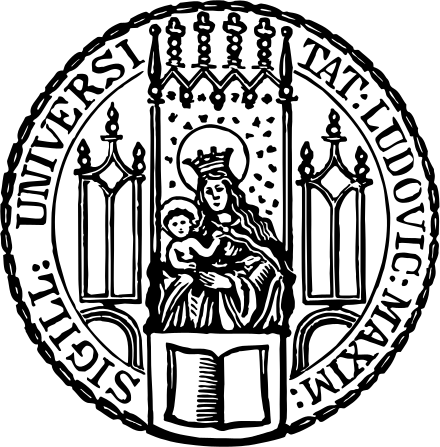
\includegraphics[scale = 0.2]{lmu_logo}
\end{flushright}
\end{minipage}%
\end{center}







\vspace{4cm}

{\centering
{
\Large\bfseries Abschlussbericht zum Projekt\\
LVS-IR-Taubenstein\par}
\vspace{9cm}
\begin{flushleft}
Projektpartner: Sascha Filimon, Roman Ossner\\ 
Gruppenbetreuer: Dr. Andr\'{e} Klima\\ 
Projektgruppe: Alexander Fogus, Lea Vanheyden, Zorana Spasojevi\'{c}
\end{flushleft}
}
\end{titlepage}



\newgeometry{top=1.25in,bottom=1.25in,right=1.25in,left=1.25in}







\vspace{5cm}















\thispagestyle{empty}







%\newpage







\begingroup

%\hypersetup{colorlinks=true, citecolor=black, linkcolor=black}

\tableofcontents

\newpage

\listoffigures

\listoftables

\setcounter{page}{1}

\thispagestyle{empty}



\endgroup



\newpage

\pagenumbering{arabic}



\chapter{Einleitung}

\setcounter{page}{1}

Als beliebtes Ziel für Touristen und Wintersportler besteht im Alpengebiet eine besondere Konfliktsituation zwischen Mensch- und Tierreich. Routen für Spaziergänger, Skifahrer und Skitourengänger grenzen oft direkt an Lebensräume von Wildtieren an und führen so zu Stress für das Wildtierreich. Die vom Deutschen Alpenverein (DAV) in Kooperation mit dem Freistaat Bayern auf den Weg gebrachte Kampagne "`Natürlich auf Tour"' soll für eine Sensibilisierung und Informationsgebung rund um das Thema Naturschutz dienen.



Neben der Aufklärung ist ein weiteres Ziel dabei, das Verhalten der menschlichen Besucher zu analysieren um daraus abzuleiten inwiefern man es womöglich steuern kann. In diesem Sinne untersuchte der DAV in Zusammenarbeit mit dem Departement für Geographie der LMU am Berg Taubenstein im Mangfallgebirge rund um den Spitzingsee in der Saison 18/19 und 19/20 den Anteil der Skitourengänger mit sogenannten LVS-Geräten. LVS-Gerät ist die Abkürzung für Lawinenverschüttetensuchgerät, mit Hilfe dieser Geräte können von Lawinen verschüttete Personen schnell gefunden werden. Personen, die ein LVS-Gerät dabeihaben, können mit diesem andere LVS-Geräte suchen und auch selbst gefunden werden.



Anhand der zur Verfügung gestellten Daten zur Saison 18/19 wird durch ein Modell der Anteil der Skitourengänger mit LVS-Gerät in Abhängigkeit von anderen Faktoren (wie z.B. Uhrzeit, Temperatur, Schneehöhe) analysiert .

Zudem wird untersucht, von welchen Einflussgrößen die Messfehler abhängen, welcher Art (Über-/Unterschätzung) sie sind und ob eine Struktur (mögl. Verteilung) vorliegt.

Unter Berücksichtigung der Erkenntnisse über die Messfehler werden Hypothesen aufgestellt, in welcher Form die Messfehler die geschätzten Abhängigkeiten beeinflussen.



Noch schreiben, was wir rausgefunden haben.



Quelle:

\url{https://de.wikipedia.org/wiki/Lawinenverschüttetensuchgerät}



\chapter{Datenbasis}

\section{Datengrundlage}

Um auf den Anteil der Skitourengängen, die ein LVS-Gerät bei sich hatten, schließen zu können, hat man Checkpoints aufgestellt. Für den Aufstieg am Taubenstein gibt es zwei Routen, eine Nord- und eine Südroute. Die genauen Lagen kann man Abbildung \ref{pic:checkpoints} entnehmen. An beiden Routen wurde jeweils ein Checkpoint aufgestellt, an dem vorbeigehende Besucher gemessen werden. Durch Infrarotmessung wird erfasst, ob ein Mensch am Checkpoint vorbeigeht. Außerdem werden LVS-Geräte, die auf Sendebetrieb geschaltet sind, erfasst. Für jede einzelne Checkpointmessung liegt das jeweilige Datum mit Uhrzeit vor und an welcher der zwei Routen (N oder S) sie erfasst wurde.



\begin{figure}[H]

\centering

\includegraphics[width=.9\textwidth]{checkpoints}

\caption{Satellitenbild, dass die Lage der zwei Routen und der Checkpoints verdeutlich}

\label{pic:checkpoints}

\end{figure}



\noindent Für die erste Untersuchung benutzen wir vorerst nur diese automatisch erfassten Daten zur Saison 18/19. Der umfasste Zeitraum läuft dabei vom 21.12.2018 bis zum 13.04.2019. Anzumerken ist dabei, dass am 23.12. und 24.12. keine Messungen vorliegen, zudem werden Messungen vom 07.01. bis zum 15.01. außer Acht gelassen, da aufgrund von starkem Schneefall die Checkpoints bedeckt waren.



Zusätzlich zu diesen automatischen Messungen wurden manuell Gruppen von (?)Studenten/Mitarbeitern des Departments für Geographie(?) an bestimmten Tagen vor Ort eingesetzt, um durch Befragungen manuelle Daten zu gewinnen. Dabei wurde festgestellt, dass bei den durch die Checkpoints erhobenen Daten Messfehler vorliegen.



Quelle:

Folien vom Erstgespräch



Neben der Erfassung von Personen und LVS-Geräten liegen verschiedene weitere Daten vor.Für jeden Tag an dem gemessen wurde gibt es Information zu den Wetterbedingungen bzw. anderen möglichen Einflussvariablen. "`snowhight"' bemisst die Schneehöhe in cm. "`temperature"' ist die Temperatur des Tages um 12:00 mittags. "`solar\_radiation"' zeigt die Sonneneinstrahlung in $W/cm^2$. Außerdem sind die Lawinenwarnstufen des jeweiligen Tages angegeben. Es kann vorkommen, dass die Lawinenwarnstufe auf der Spitze des Berges eine andere ist als im Tal, deshalb gibt es zwei Variablen: "`avalanche\_report\_top"' und "`avalanche\_report\_down"'. Diese geben die Lawinenwarnstufe an der Spitze und am Fuß des Berges an. Obwohl es Stufen von 1 (niedrig) bis 5 (sehr hoch) gibt, war die in dem beobachteten Zeitraum höchste Stufe eine 4. An Tagen an denen die Stufen unterschiedlich waren wurde außerdem in "`avalanche\_report\_border"' der Höhenmeter angegeben, ab dem sich die Lawinengefahr unterscheidet. In "`avalanche\_report\_comment"' ist vermerkt, ob es sich dabei um eine Waldgrenze handelt. "`day"' gibt an, um welchen Tag der Woche es sich handelt und "`day\_weekday"', "`day\_weekend"' und "`holiday"' geben jeweils an, ob der Tag ein Tag unter der Woche oder am Wochenende war und ob er sich innerhalb einer Ferienzeit befunden hat.



\section{Datenaufbereitung}

Der erste Schritt besteht darin, die gegebenen Daten um weitere 

Bearbeitung der Daten durch uns:

(noch mehr schreiben)

sunnrise und sunset

"`count\_beacon"' und "`count\_infrared"' enthalten die Anzahl der gemessenen LVS-Geräte bzw. Infrarotmessungen pro Tag.

Umwandlung der Messungen zu Personendaten. Umstellung des Tages von 04:00 bis 04:00.

Eine Übersicht über alle Variablen die verwendet wurden ist in Tabelle \ref{tab:var} zu finden.





\begin{table}

\centering

\caption{Übersicht aller benutzten Variablen mit kurzer Beschreibung}

\begin{adjustbox}{max width=\textwidth}

\begin{tabular}{l|l|l}

\textbf{Name} & \textbf{Beschreibung} & \textbf{Werte} \\

\hline

\hline

date & Datum & Datum vom 25.12.2018 bis zum 15.01.2019 \\

\hline

time & Uhrzeit(minutengenau) & Uhrzeit von 03:59 bis 03:59 \\

\hline

position & Route an der gemessen wurde & diskret (2 Ausprägungen): S,N \\

\hline

lvs & Hat die gemessene Person ein LVS-Gerät mitgeführt? & diskret (2 Auspr.): ja, nein \\

\hline

day & Wochentag & diskret (7 Auspr.): Montag, Dienstag,... \\

\hline

snowhight & Schneehöhe in cm (am Tag der Messung) & stetig: 16-212 \\

\hline

temperature & Temperatur in °C um 12:00 & stetig: (-7.9)-(9.7) \\

\hline

solar\_radiation & Sonneneinstrahlung in $W/cm^2$ & stetig: 14-792 \\

\hline

avalanche\_report & berechnete Lawinenwarnstufe & diskret (7 Auspr.): 1, 1.5, 2,... \\

\hline

holiday & Handelte es sich um einen Ferientag? & diskret (2 Auspr.): ja, nein \\

\hline

sunrise & Uhrzeit des Sonnenaufgangs & Uhrzeit von 05:29 bis 08:02 \\

\hline

sunset & Uhrzeit des Sonnenuntergangs & Uhrzeit von 16:24 bis 18:58 \\

\hline

day\_length & berechnete Länge des Tages (von Sonnenauf- bis Sonnenuntergang) & von 08:24 bis 13:28 h \\

\hline

\end{tabular}

\end{adjustbox}

\label{tab:var}

\end{table}



\chapter{Deskriptive Analyse}

Insgesamt 37593 Messungen an 114 Tagen



8468 Beacons, 29125 Infrareds (vor Umkodierung)



nach Umkodierung: 31574 Personen



8468 mit LVS-Gerät, 23106 ohne LVS-Gerät

pr

Die meisten Leute zwischen 09:00 und 18:00 unterwegs



--



Schneehöhe nimmt bis Mitte Januar stark zu und fällt ab Mitte Februar ab



Temperatur nimmt im Trend bus Mitte Januar ab und steigt danach



Sonnenstrahlung steigt bis März leicht und danach stark





---





Anteil schwankt in den ersten Wochen deutlich



generell viele Ausreißer, aber kein große Veränderung bei Schneehöhe, Temperatur und Sonneneinstrahlung



Anteile zur Mittagszeit geringer



mit steigender Lawinengefahr steigt die Anzahl



\chapter{Methodik}
In folgendem Kapitel soll in einem Modell der Zusammenhang einer beobachteten abhängigen Variable, in unserem Fall, der Anteil der Skitourengänger mit LVS-Gerät, durch mehrere unabhängige Variablen erklärt werden.
Mithilfe der generalisierten additiven Regression lässt sich diese Fragestellung auf eine flexible und strukturierte Weise lösen. Die Modellierung wird mittels nichparametrischer Regression durchgeführt.
Dabei wird im ersten Schritt eine einfache nichtparametrische Regression mit normalverteilter Zielvariable und einer einzigen Kovariable angenommen. Die Modellierung dient zu Veranschaulichung der Polynom- und Penalisierungs-Splines, sowie deren Basisfunktion. Im letzten Schritt wird die Modellierung der Splines mit dem generalisierten additiven Modell verknüpft und durch ein Modell mit mehreren Kovariablen erweitert. Die mathematischen Formeln und Konzepte aus diesem Kapitel basieren, wenn nicht anders vermerkt, aus dem Buch \glqq{Regression-Modelle, Methoden und Anwendungen}\grqq ~von Ludwig Fahrmeir. 

\section{Nichtparametrische Regression}
Bei einem linearen Regressionsmodell wird der Erwartungswert einer Zielvariable durch die Linearkombination von Einflussgrö"sen, auch Kovariablen genannt, beschrieben. In praktischen Anwendungen ist dies oft unzureichend, da neben den linearen Einflüssen auch nicht-lineare, flexible Einflüsse von stetigen Kovariablen auf die abhängige Variable wirken können.
Die univariate Glättung stellt ein Verfahren dar, welche eine fexible Modellierung genau einer metrischen unabhängigen Variable auf eine metrische Zielvariable ermöglicht. Es wird davon ausgegangen, dass die Messungen $(y_{i},z_{i})$ mit $i=1,...,n$ gegeben sind, wobei $y_{i}$ die Beobachtungen der Zielvariable und $z_{i}$ die Werte eine metrischen Kovariable abbilden. Die Zielvariable soll nun durch eine Funktion der Kovariable und einen additiven Störterm ($\epsilon_{i}$) erklärt werden:

\begin{align}
y_{i}=f(z_{i})+\epsilon_{i};\enspace E(\epsilon_{i})=0 \enspace und \enspace Var(\epsilon_{i})=\sigma^2 \enspace mit \enspace i=1,...,n.
\end{align}

Daraus ergibt sich:

\begin{align}
E(y_{i})=f(z_{i}) \enspace Var(y_{i})=\sigma^2 \enspace mit \enspace i=1,...,n,
\end{align}
was bedeutet, dass die Schätzfunktion $f$ den Erwartungswert der abhängigen Variable darstellt.

\subsection{Polynom-Splines}

Eine Möglichkeit, die Funktion $f$ abzubilden, sind Splines, die über Polynome modelliert werden und Polynom-Splines, oder auch Regressions-Splines, genannt werden. Das polynomiale Modell hat die Form: 
\begin{align}
f(z)=\gamma_{0}+\gamma_{1}z+...+\gamma_{l}z^l,
\end{align}
wobei das Polynom vom Grad $l$ durch den Einfluss von $z$ auf $y$ modelliert wird und $\gamma_{j}$ die Regressionskoeffizienten darstellen. Um eine flexible Schätzfunktion gewährleisten zu können, wird der Definitionsbereich von $z$ in Intervalle geteilt und Polynome werden für das jeweilige Intervall geschätzt. Die Zerlegung von $z$ erfolgt stückweise auf Basis von sogenannten Knotenmengen $k_{1}$ bis $k_{m}$.  Ein Problem, welches dabei entstehen könnte ist, dass an den Intervallgrenzen keine $glatte$ Funktion entstehen. Der Graph einer $glatten$ Funktion hat an den Intervallgrenzen keine \glqq{Ecken\grqq}. Deshalb muss für die \glqq{mathematische}\grqq ~Glattheit die zusätzliche Bedingung, dass die Funktion $f(z)$ an den Intervallgrenzen $(l-1)$-mal stetig differenzierbar ist, eingeführt werden. Der Grad des Splines und die Anzahl der Knoten können somit im hohen Ma"se die Funktion beeinflussen, je höher die Anzahl an Knoten ist, desto $rauer$ ist die Funktion $f(z)$. Um Polynom-Splines in der Praxis anwenden zu können, bedarf es einer Darstellung der Menge der Polynom-Splines. Eine mögliche Darstellung eines Polynom-Splines stellt die B-Spline-Basisfunktion dar.

\subsection{Basis Splines (B-Splines)}
Der B-Spline dient als Basisfunktion für Polynom-Splines. Jedoch wird sich auch der Penalisierungs-Spline, welcher im darauffolgenen Kapitel vorgestellt wird, die B-Spline-Basisfunktion zu Nutzen machen. Das Ziel bei der Konstruktion der B-Spline-Basisfunktion ist es die Polynomstücke des gewünschten Grades an den Knoten ausreichend $glatt$ zusammenzusetzen. Die Basisfunktion besteht dabei aus $(l+1)$ Polynomstücken vom Grad $l$, welche stetig an den Knoten zusammengesetzt werden. Die Funktion $f(z)$ lässt sich durch die Linearkombination der Basisfunktionen:
\begin{align}
f(z)=\sum_{j=1}^d\gamma_{j}B_{j}(z)
\end{align}
darstellen. Die Koeffizienten  $\gamma_{j}$ werden mit Hilfe der KQ-Methode geschätzt und dienen zur Skalierung der Basisfunktionen. Die Anzahl der erforderlichen Basisfunktionen $d = m+l-1$, setzt sich aus der Zahl der Knoten $m$ und den Polynomstücken des gewünschten Grades $l$, welche $(l-1)$-mal stetig differenzierbar an den Knoten aneinandergefügt werden, zusammen.  \\
Für B-Splines vom Grad 0 folgt:
\begin{align}
B_{j}^0(z)= \mathbb{1}_{[k_{j},k_{j+1}]}(z)= 
\begin{cases}
1 & k_{j} \leq z<k_{j+1};\enspace mit\enspace j=1,...,d-1; \\
0 & \text{sonst.} \\
\end{cases}
\end{align}
Für B-Splines höheren Grades gilt:
\begin{align}
B_{j}^l(z)= \frac{z-k_{j}}{k_{j+l}-k_{j}}B_{j}^{l-1}(z)+
\frac{k_{j+l+1}-z}{k_{j+l+1}-k_j+1}B_{j+1}^{l-1}(z).
\end{align}
Die Abbildung \ref{pic:b_spline} visualisiert die Schätzung eines B-Splines anhand eines fiktiven Datenbeispiels schematisch. Abbildung (a) demonstriert eine B-Spline Basis vom dritten Grad. In Abbildung (b) wird die Basisfunktion mit dem Kleinste-Quadrate-Schätzer $\hat\gamma_{j}$ skaliert. Die Abbildung (c), zeigt die erhaltene Schätzung, wenn die skalierten Basisfunktionen addiert werden.
\begin{figure}[H]
\centering
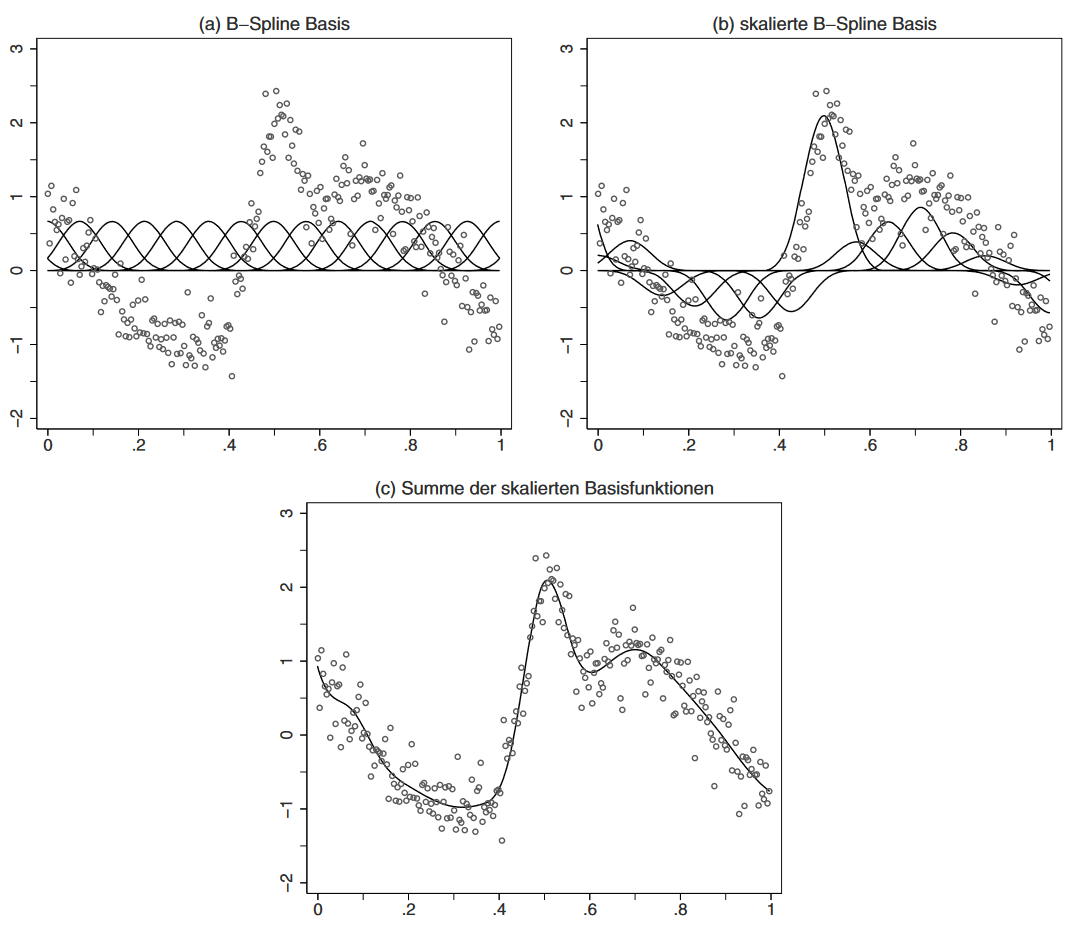
\includegraphics[width=.9\textwidth]{b_spline}
\caption{Schematische Darstellung der Schätzung eines nichtparametrischen Effekts mit B-Splines}
\label{pic:b_spline}
\end{figure}

\noindent Das nächste Kapitel behandelt P-Splines, welche auf B-Splines basieren und durch einen Strafterm erweitert worden sind. In unserer Arbeit beschränken wir uns auf P-Splines.



\subsection{Penalisierte Splines basierend auf B-Splines} 
Im vorherigen Kapitel, haben wir die Wichtigkeit der Knotenmenge kennengelernt. Die Glattheit und Flexibilität der Schätzfunktion $f(z)$ hängt stark von der Anzahl der Knoten ab. Das Ziel ist es die Funktion $f(z)$ auf Basis einer B-Spline Funktion, mit einer großen Zahl an Knoten, zu approximieren um so die Flexibilität der Schätzfunktion sicherzustellen und andererseits zu hohe Variabilität in Form eines Strafterms zu sanktionieren. Der Penalisierte-Spline, gekürzt P-Spline, kombiniert somit eine B-Spline-Basis verbunden mit einem Strafterm. Der Strafterm für B-Splines wird häufig durch die quadrierte zweite Ableitung der Schätzfunktion $f(z)$ modelliert, da diese Form im R-Paket $mgcv$ von Simon Woods implementiert wird. Die zweite Ableitung stellt ein Maß für die Krümmung der Funktion dar und ist daher in der Lage die Glattheit einer Funktion einzuschätzen.
Der Strafterm: 
\begin{align}
\lambda\int(f''(z))^2dz
\end{align}
beruht auf der quadrierten zweiten Ableitung der Schätz-Funktion, welche nach $z$ integriert wird und durch den Glättungsparameter $\lambda$ dargestellt wird. Die Glattheit der Schätzung des Modells im penalisierten Fall, wird primär durch den Glättungsparameter ($\lambda$) reguliert, d.h. je grö"ser $\lambda$, desto glatter ist die Schätzung.\\



\noindent\textbf{Zyklische P-Splines} \\
Eine Glättungsfunktion hei"st $zyklisch$, wenn die Funktion dieselben Werte und ersten Ableitungen an ihrer oberen und unteren Grenze aufweist. Beispielsweise kann man die Funktion für die Variable Woche mit Hilfe von zyklische P-Splines modellieren. So könnte man sicher stellen, dass die Werte am Ende einer Woche zusammenhängend zu den Werten am Anfang der Woche sind. Beispielsweise könnte der Fall eintreten, dass Werte von Sonntag den Wert von Montag beeinflussen und andersherum. Der Penalisierungsansatz für zyklische P-Splines ist simultan zu der Penalisierung von P-Splines basierend auf B-Splines (siehe 4.6) \\

(\textbf{Simon Woods Buch in Bib leihen und Zyklische Splines weiter ausführen})


\section{Additives Modell}
In diesem Kapitel, werden wir vom einfachen Modell mit normalverteilter Zielvariable und genau einer Kovariable, auf ein additives Modell mit mehreren Kovariablen übergehen. Das additive Modell stellt in der Statistik ein nicht-parametrisches Regressionsmodell dar. Neben mehreren nicht-linearen flexiblen Einflüssen können hier auch lineare Einflüsse von Kovariablen auf die abhängige Variable modelliert werden. \\
Das Standardmodell der additiven Regression (ohne Interaktionen) hat die Form:
\begin{align} 
y_{i}=\underbrace{f_{1}(z_{i1})+...+f_{q}(z_{iq})}_{\text{nicht-parametrische Effekte}}+\underbrace{\beta_{0}+\beta_{1}x_{i1}+...+\beta_{k}x_{ik}}_{\text{parametrische Effekte}}+\epsilon_{i}
\end{align}
Die Funktionen $f_{1}(z_{1}),...,f_{q}(z_{q})$ werden mit nichtparametrischen Effekten, die wir bereits im vorherigen Kapitel (4.1) erläutert haben, geschätzt. Der Störterm besitzt die gleichen Annahmen, wie das einfache Modell mit nur einer Kovariable. Das Modell (4.8) kann durch Interaktionseffekte erweitert werden um Wechselwirkungen zwischen den Kovariablen zu integrieren. Seien $z_{1}$ und $z_{2}$ metrische Variablen, dann ergibt sich durch das additive Einbeziehen der Prädiktor:
\begin{align}
\eta_{i}=f_{1}(z_{i1})+f_{2}(z_{i2})+f_{1,2}(z_{i1},z_{i2})+...,
\end{align}
welcher durch die zweidimensionale Funktion $f_{1,2}(z_{1},z_{2})$ erweitert wurde. Die Schätzung der Funktion $f_{1,2}(z_{1},z_{2})$ erfolgt über eine nichtparametrische bivariate Methode. 
\subsection{Generalisierte additive Modell}
Nichtlineare Effekte von metrischen Kovariablen treten auch bei Regressionsmodellen auf, die keine normalverteilte Zielvariable haben. Die abhängige Variable nimmt aber typischerweise eine Verteilung aus einer Exponentialfamilie (z.B. Binomial, Poisson, Multinomial, Normal,...) an.  In unserem Fall, handelt es sich um eine binär verteilte Zielvariable, die sich folgenderma"sen darstellen lässt:
\begin{align}
y_{i}=\begin{cases}
1 & \text{,wenn Person mit LVS-Gerät identifiziert wird } \\
0 & \text{,wenn Person ohne Lvs-Gerät identifiziert wird.} \\
\end{cases}
\end{align}
Allgemein sieht das generalisierte additive Modell mit binär verteilter Zielvariable,\enspace $y_{i}|x_{i}\sim B(1,\pi_{i})$, folgenderma"sen aus.
Der Erwartungswert $\mu$ der Zielvariable $y$ wird mit dem additiven Prädiktor:
\begin{align}
\eta_{i}= f_{1}(z_{i1})+...+f_{q}(z_{iq})+\beta_{0}+\beta_{1}x_{i1}+...+\beta_{k}x_{ik},
\end{align}
durch eine Responsefunktion $h$ bzw. eine Linkfunktion $g=h^{-1}$ zu:
\begin{align}
\mu=h(\eta) ~bzw. \eta=g(\mu)
\end{align}
verknüpft.
Dabei ist der Prädiktor ein wichtiges Hilfsmittel bei der effizienten Codierung von additiven Modellen. Wie schon im vorherigen Kapitel (4.1) beschrieben, sind $f_{1}(z_{i1}),...,f_{q}(z_{iq})$ $glatte$ Funktionen, die grundsätzlich nicht durch eine starre parametrische Form festgelegt werden, sondern durch nicht-parametrische Methoden geschätzt werden. Die Parameter $\beta_{0},...,\beta_{k}$ werden mittels der Maximum-Likelihood-Methode:
\begin{align}
L(\beta)=\prod_{i=1}^{n}L_{i}(\beta)=\prod_{i=1}^{n}\pi_{i}^{y_{i}}(1-\pi_{i})^{1-y_{i}}
\end{align}
bestimmt. \\
Für den Erwartungswert der Zielvariable gilt:
\begin{align}
E(y_{i})=\pi_{i}=\frac{exp(\eta_{i})}{1+exp(\eta_{i})}.
\end{align}
Dies lässt sich mit dem Logit-Link zu
\begin{align}
\log(\pi_{i})=\log(\frac{\pi_{i}}{1-\pi_{i}})
\end{align}
trasformieren. \\
Des weiteren muss die Varianzhomogenität, auch Homoskedastizität genannt, nicht unbedingt befriedigt sein. Das hei"st, die Varianz ist in einigen Fällen nicht konstant und hat die Form:
\begin{align}
Var(y_{i})=\frac{\pi_{i}(1-\pi_{i})}{w}.
\end{align}
Der Gewichtungsfaktor $w$ wurde eingeführt um den Fall von Individual- und gruppierten-Daten gleich zu behandeln. Für Individualdaten gilt $w=1$, für gruppierte Daten nimmt $w$ den Umfang der Gruppe an. Auf die Bedeutung von gruppierten Daten, wird im nächsten Kapitel näher eingegangen. 
Beim Störterm $\epsilon_{i}$ geht man davon aus, dass dieser unabhängig sein muss, jedoch ist $\epsilon_{i}$ im binären Fall nicht normalverteilt. \\
(Quelle von Störterm: https:\//online.stat.psu.edu\/stat504\/node\/220\/)
\section{Gruppierte Daten}
\section{Dispersion}
\textbf{Überdispersion} \\
Die Überdispersion beschreibt ein wichtiges Konzept. Für gruppierte Daten lässt sich die Varianz innerhalb der Gruppe abschätzen. In Anwendungen ist diese \textit{empirische} Varianz oft deutlich größer als die durch ein binomiales Regressionsmodell vorhergesagte Varianz. Eine mögliche Lösung dafür, wäre die Einführung eines multiplikativen Überdispersionsparameters $\phi > 1$ in die Varianzformel, d.h.
\begin{align}
Var(y_{i}|\textbf{x}_{i})=\phi \frac{\pi_{i}(1-\pi_{i})}{n_{i}}.
\end{align}
(Quelle von Modell-Fit: https:\//online.stat.psu.edu\/stat504\/node\/220\/) \\
(Quelle von Überdispersion: Fahrmeir Regression)


\end{document}
